\paragraph\indent ReSP~\cite{fossati_resp} is an MPSoC simulation platform working at a high abstraction level. It provides a non-intrusive framework to manipulate its components based on SystemC~\cite{arnout_systemc_2000}, TLM~\cite{cai_transaction_2003,osci_tlm}, and communication description libraries. The simulation platform is built using Python programming language; its reflective capabilities augment the platform with the possibility of observing the internal structure of the SystemC component models. This feature enables run-time composition and dynamic management of the architecture under analysis. The full potentialities offered by the integration among Python and SystemC are exploited, during simulation, to query, examine and, possibly, modify the internal status of the hardware models. These capabilities simplify the debugging process for both the modeled hardware architecture and the software running on it.

\section{Features}
\label{intro:feat}
\paragraph\indent The ReSP simulation platform currently contains the following features:
\begin{description}
  \item[Components Library]: the aim of this work, as explained later, is not to build a rich library of SystemC models, but rather to create efficient mechanisms through which these components can be connected, analyzed and through which simulation can be efficiently managed. Anyway we built some component models of processors, buses and various peripherals; later follows a detailed description of them.
  \item[Seamless Integration] of new components inside the simulator itself; this is achieved thanks to the reflective capabilities of ReSP, which are obtained through the automatic creation of Python Wrappers around the SystemC models.
  %\item[GDB]: the GDB debugger is integrated within the processor simulators and the memory interfaces; there is anyway a loose coupling among the ISS and GDB, so that adding a new processor model is just a matter of specifying how the ISS variables maps to the physical real processor registers. With our GDB stub it is possible to use the majority of GDB native functionalities and commands in order to debug your program. The stub has been designed to support coordination among processors in case multi-processor architectures are used. In addition to all this, some additional commands (accessible using the \texttt{monitor} GDB command) are created in order to manage simulation time.
  %\item[Debugging Tools]: we developed some tools which might help the programmer in discovering bugs inside their programs. In particular we concentrated on the Memory Analyzer, used after simulation ended to examine the state of the memory in every simulation instant; it has also the possibility of performing simple queries on the memory history. Additional tools such as a Tracer or a Profiler could be simply instrumented for the processors and transaction level interconnections in order to obtain a trace or to profile an execution.
  \item[OS Emulation]: ReSP has the possibility of completely emulating a multi-threaded multi-processor posix-compilant Operating System. This means that every call to Operating System routines performed by your program (the one running on the ISS) will be forwarded to the host OS (the one running on your PC) instead of being simulated. Thanks to the cross-compilation of the \texttt{libgomp} library it is also possible to emulate OpenMP based programs.
  \item[Binutils Wrapper]: instantiated around the \texttt{binutils} libraries (in particular around BFD) in order to be able to access, parse and, in case, modify executable files. This wrapper is currently used for the OS emulation; furthermore, it can be used also for deugging purposes.
  \item[Cross-Compilers]: are furnished in order to compile the applications running on the Instruction Set Simulators. They are based on \texttt{newlib} and fully support our OS emulation mechanism.
  \item[TCP interface]: in order to be able to control ReSP through a socket interface. This interface can be used by an external program (for example a GUI) to communicate with ReSP.
\end{description}

\section{Problems of current simulators}
\label{intro:problems}
\paragraph\indent Most (if not all) of the most successful hardware simulators are based on SystemC and TLM libraries; these libraries are written using the C++ language, thus these simulators have both the advantages and disadvantages of this language:
\begin{itemize}
  \item[+] Execution Speed (if compared for example to languages such as Java, etc.)
  \item[+] Object Oriented Programming Style (which consistently clarifies the written code)
  \item[-] The hardware components to be plugged into the simulator need to inherit from specific interfaces (i.e. they need to have particular methods and attributes which must be known to the simulator itself) in order for the simulator to be able to use them.
\end{itemize}
\indent Switching to languages such as Java creates two problems: first of all no library (such as SystemC is for C++) for the description of hardware systems exists for these languages; moreover execution speed of the languages is terribly slow: given that even C++ simulations can last for days, Java ones can even take months. On the other hand, reflection (the capability of a program of viewing and modifying the structure of the program itself) is a property of interpreted languages (such as Java, C\# or Python). Through reflection, a simulator is able to determine, at runtime, which are the methods that need to be called in order to connect together heterogeneous components, to initialize them, to read their internal status. This is done without the need for the simulator to have any a-priory knowledge on the structure of the components themselves.\\
\indent ReSP tries to combine the reflection property of interpreted languages (such as Java or Python) together with execution speed of C++ and expressiveness of SystemC. This is done by using C++ and SystemC for the computational part of the simulation, while the connection of the components and the inspection of their internal status is done by using Python.

\section{ReSP: Reflective Simulation Platform}
\label{intro:resp}
\paragraph\indent The simulation platform itself is built using Python programming language; its reflective capabilities augment the platform with the possibility of observing the internal structure of the SystemC component models. This feature enables run-time composition and dynamic management of the architecture under analysis. The full potentialities offered by the integration among Python and SystemC are exploited, during simulation, to query, examine and, possibly, modify the internal status of the hardware models. These capabilities simplify the debugging process for both the modeled hardware architecture and the software running on it.\\
\indent The advantages of coupling standard SystemC based simulation techniques together with the reflective capabilities of Python are multiple:
\begin{enumerate}
  \item introspection inside the components, which simplifies the integration of external IPs.
  \item fine grain control of the simulation, allowing an easy monitoring and modification of the status of the components.
  \item effortless integration of new tools for the analysis and the design space exploration; for instance, the simulator has been extended with features for system reliability assessment.
\end{enumerate}
\indent The integration among Python and C++ is achieved through wrappers: they are written in C++ and they allow Python to query, modify and instantiate C++ objects; the burden of writing these wrappers is not on the programmer, but they are automatically created: the generation flow is shown in Figure~\ref{intro:resp:wrapper}.\\
\begin{figure}
\begin{center}
  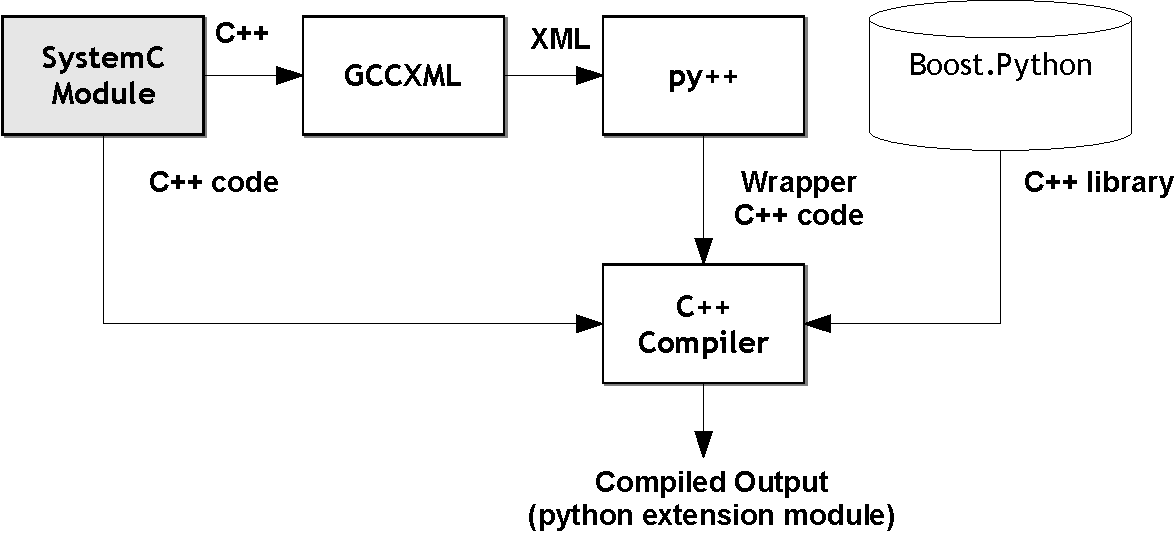
\includegraphics[width=\columnwidth]{resp-wrapperflow}
\end{center}
\caption{ReSP wrapper Generation}
\label{intro:resp:wrapper}
\end{figure}
\indent Each header file is parsed using GCCXML, a tool that provides an XML description of GCC abstract syntax tree (i.e. GCCXML produces an XML file containing the description of the classes, methods, etc. of the cpp source files; for example, for each class, the XML file contains the class name, the list of its attributes, the list of methods, etc.). The resulting XML description
is manipulated to select all the parts that need to be exported (i.e. made visible to Python), and then the OpenSource tool \texttt{py++} is used to generate Python wrapping code that uses the \texttt{Boost.Python} library. The advantage of Boost.Python and py++ over alternative tools like \texttt{SWIG} (used by most other works) is that it guarantees access to all C++ declarations, even private or protected ones, through the generation of appropriate class wrappers. The Python interpreter can load the extensions generated by the ReSP flow, and have full access to the C++, and therefore SystemC, classes contained in the exported module. Another feature of the ReSP flow is that IP documentation is automatically extracted from the SystemC source code, and inserted in
the Python wrapper. Python self-documentation features are then used to display such documentation through the User Interface.

\section{Document Outline}
\paragraph\indent This guide will show how to use the ReSP simulation platform in order to describe, simulate and analyze simple hardware architectures while running standard pieces of software cross-compiled for the specific platforms. This Chapter introduced the main idea behind this simulation platform. Starting from Chapter~\ref{install} the user will be taught how to install the tool; then, on Chapter~\ref{general} the basic use of the platform will be described and shown through some practical examples; afterwards, Chapters~\ref{reconfigurable} and~\ref{fault} will introduce some specific uses of the simulation platform while dealing with reconfigurable components and fault analysis; finally, Chapter~\ref{describe} is going to offer the basis for the development of new hardware components inside the ReSP simulation platform.
